\clearpage
\subsection{National input tables}
\label{app:eda-national-inputs}
\begin{mergedcontribution}{authorSowmya}
Table~\ref{tab:o1-periods} groups the monthly observations into four periods, separated by the Jet Airways exit in April 2019, Tata's acquisition of Air India in January 2022 and the late-2024 mergers. These are period means rather than individual monthly observations.

\begin{minipage}{\linewidth}
\captionsetup{font={small,color=authorSowmya},labelfont=bf,justification=raggedright,singlelinecheck=false,hypcap=false}
\captionof{table}{O1: Concentration measures by period (period means).}
\label{tab:o1-periods}
\centering
{\small\setstretch{1.1}\setlength{\tabcolsep}{4pt}
\fontsize{10}{12}\selectfont\setstretch{1}\setlength{\tabcolsep}{3pt}
\renewcommand{\arraystretch}{1.15}
\begin{tabular}{|>{\raggedright\arraybackslash}p{\dimexpr0.28\linewidth-2\tabcolsep-1.1428571428571428\arrayrulewidth\relax}|>{\raggedright\arraybackslash}p{\dimexpr0.12\linewidth-2\tabcolsep-1.1428571428571428\arrayrulewidth\relax}|>{\raggedright\arraybackslash}p{\dimexpr0.12\linewidth-2\tabcolsep-1.1428571428571428\arrayrulewidth\relax}|>{\raggedright\arraybackslash}p{\dimexpr0.12\linewidth-2\tabcolsep-1.1428571428571428\arrayrulewidth\relax}|>{\raggedright\arraybackslash}p{\dimexpr0.12\linewidth-2\tabcolsep-1.1428571428571428\arrayrulewidth\relax}|>{\raggedright\arraybackslash}p{\dimexpr0.12\linewidth-2\tabcolsep-1.1428571428571428\arrayrulewidth\relax}|>{\raggedright\arraybackslash}p{\dimexpr0.12\linewidth-2\tabcolsep-1.1428571428571428\arrayrulewidth\relax}|}
\hline
\textbf{Period} & \textbf{Brand HHI} & \textbf{Own.\ HHI} & \textbf{MHHI} & \textbf{CR2 (\%)} & \textbf{Gap (pp)} & \textbf{Fringe (\%)} \\
\hline
Pre-Jet exit (Jan 2015--Apr 2019) & 2{,}323.8 & 2{,}408.0 & 2{,}416.1 & 58.7 & 21.8 & 41.3 \\
\hline
Jet exit to Tata (May 2019--Dec 2021) & 3{,}293.1 & 3{,}294.5 & 3{,}342.3 & 66.9 & 39.2 & 33.1 \\
\hline
Tata to mergers (Jan 2022--Nov 2024) & 3{,}847.6 & 4{,}308.6 & 4{,}308.6 & 85.5 & 33.1 & 14.5 \\
\hline
Post mergers (Dec 2024--Jul 2026) & 4{,}538.0 & 4{,}876.7 & 4{,}876.7 & 90.7 & 38.0 & 9.3 \\
\hline
\end{tabular}\par}
\vspace{4pt}
{\footnotesize\setstretch{1.1}\raggedright\textit{Note:} HHI values are index points; CR2, gap and fringe use ownership-group passenger shares. April 2020 is missing and not imputed.\par
\textit{Source:} DGCA monthly airline traffic via \href{https://github.com/mkubicek/india-aviation-stats/tree/16770ac59dae61ce7b80fd8bd67dd7f4cef280a6}{Kubicek (2026)}; authors' calculations.\par}
\end{minipage}
\end{mergedcontribution}
\begin{mergedcontribution}{authorMeena}
The brands brought under one owner in January 2022 held 22.5\% of passengers, and those merged in late 2024 held 29.3\% (Table~\ref{tab:o2-tata}). These shares are the inputs to the mechanical \HHI{} calculation in Section~\ref{sec:o2-results}.

\begin{table}[H]
\centering
\color{authorMeena}
\caption{Passenger shares of the Tata brands before each consolidation step (\%)}\label{tab:o2-tata}
\small
\fontsize{10}{12}\selectfont\setstretch{1}\setlength{\tabcolsep}{3pt}
\renewcommand{\arraystretch}{1.15}
\begin{tabular}{|>{\raggedright\arraybackslash}p{\dimexpr0.32\linewidth-2\tabcolsep-1.1666666666666667\arrayrulewidth\relax}|>{\raggedright\arraybackslash}p{\dimexpr0.13\linewidth-2\tabcolsep-1.1666666666666667\arrayrulewidth\relax}|>{\raggedright\arraybackslash}p{\dimexpr0.14\linewidth-2\tabcolsep-1.1666666666666667\arrayrulewidth\relax}|>{\raggedright\arraybackslash}p{\dimexpr0.12\linewidth-2\tabcolsep-1.1666666666666667\arrayrulewidth\relax}|>{\raggedright\arraybackslash}p{\dimexpr0.18\linewidth-2\tabcolsep-1.1666666666666667\arrayrulewidth\relax}|>{\raggedright\arraybackslash}p{\dimexpr0.11\linewidth-2\tabcolsep-1.1666666666666667\arrayrulewidth\relax}|}
\hline
\textbf{Step (shares in)} & \textbf{Air India} & \textbf{AI Express} & \textbf{Vistara} & \textbf{AirAsia India\textsuperscript{a}} & \textbf{Total} \\
\hline
Acquisition, Jan 2022 (Dec 2021) & 8.39 & 0.07 & 7.72 & 6.28 & 22.46 \\
\hline
Mergers, Dec 2024 (Sep 2024) & 11.14 & 3.97 & 10.04 & 4.11 & 29.26 \\
\hline
\end{tabular}
\sourcenote{DGCA monthly airline statistics via \textcite{kubicek2026aviationstats}; authors' calculations. \textsuperscript{a}Renamed AIX Connect. September 2024 is the last month before the AIX Connect merger (October 2024) and the Vistara merger (November 2024).}
\end{table}

The market grew in both post-exit windows, with passengers rising faster than seat-km, so rivals mainly filled existing seats (Table~\ref{tab:o2-market}).

\begin{table}[H]
\centering
\color{authorMeena}
\caption{Market size and capacity before and after each exit (monthly averages)}\label{tab:o2-market}
\small
\setlength{\tabcolsep}{5pt}
\fontsize{10}{12}\selectfont\setstretch{1}\setlength{\tabcolsep}{3pt}
\renewcommand{\arraystretch}{1.15}
\begin{tabular}{|>{\raggedright\arraybackslash}p{\dimexpr0.12\linewidth-2\tabcolsep-1.1666666666666667\arrayrulewidth\relax}|>{\raggedright\arraybackslash}p{\dimexpr0.24\linewidth-2\tabcolsep-1.1666666666666667\arrayrulewidth\relax}|>{\raggedright\arraybackslash}p{\dimexpr0.16\linewidth-2\tabcolsep-1.1666666666666667\arrayrulewidth\relax}|>{\raggedright\arraybackslash}p{\dimexpr0.17\linewidth-2\tabcolsep-1.1666666666666667\arrayrulewidth\relax}|>{\raggedright\arraybackslash}p{\dimexpr0.13\linewidth-2\tabcolsep-1.1666666666666667\arrayrulewidth\relax}|>{\raggedright\arraybackslash}p{\dimexpr0.18\linewidth-2\tabcolsep-1.1666666666666667\arrayrulewidth\relax}|}
\hline
\textbf{Exit} & \textbf{Window} & \textbf{Passengers (million)} & \textbf{Capacity (billion seat-km)} & \textbf{Load factor (\%)} & \textbf{Average no. of groups with $\geq$1\% share} \\
\hline
Jet Airways & Apr 2018--Mar 2019 & 11.69 & 13.07 & 86.0 & 8.0 \\
\hline
 & May 2019--Feb 2020 & 12.25 & 13.60 & 87.1 & 7.0 \\
\hline
Go First & May 2022--Apr 2023 & 11.53 & 13.29 & 84.1 & 5.6 \\
\hline
 & Jun 2023--May 2024 & 12.88 & 14.25 & 87.2 & 4.6 \\
\hline
\end{tabular}
\sourcenote{DGCA monthly airline statistics via \textcite{kubicek2026aviationstats}; authors' calculations. Capacity (seat-km) $=$ seats offered $\times$ kilometres flown. Load factor $= 100 \times \dfrac{\text{passenger-km}}{\text{seat-km}}$, the share of seats filled.}
\end{table}
\end{mergedcontribution}
\begin{mergedcontribution}{authorGoutham}
\begin{samepage}
Between December 2024 and December 2025, rivals' offered capacity rises from 6.385 to 6.619 billion seat-kilometres, while passenger traffic rises from 5.493 to 5.947 billion passenger-kilometres. Table~\ref{tab:o4-capacity-inputs} gives the complete inputs.

\begin{minipage}{\linewidth}
\captionsetup{font=small,labelfont=bf,justification=raggedright,singlelinecheck=false,hypcap=false}
\captionof{table}{Capacity and passenger-traffic inputs for the December comparison.}
\label{tab:o4-capacity-inputs}
\centering
{\small\setstretch{1.1}\fontsize{10}{12}\selectfont\setstretch{1}\setlength{\tabcolsep}{3pt}
\renewcommand{\arraystretch}{1.15}
\begin{tabular}{|>{\raggedright\arraybackslash}p{\dimexpr0.17\linewidth-2\tabcolsep-1.25\arrayrulewidth\relax}|>{\raggedright\arraybackslash}p{\dimexpr0.21\linewidth-2\tabcolsep-1.25\arrayrulewidth\relax}|>{\raggedright\arraybackslash}p{\dimexpr0.31\linewidth-2\tabcolsep-1.25\arrayrulewidth\relax}|>{\raggedright\arraybackslash}p{\dimexpr0.31\linewidth-2\tabcolsep-1.25\arrayrulewidth\relax}|}
\hline
\textbf{Month} & \textbf{Airlines} & \textbf{Offered capacity (billion seat-km)} & \textbf{Passenger traffic (billion passenger-km)} \\
\hline
Dec 2024 & IndiGo & 10.053 & 9.113 \\
\hline
Dec 2024 & Other airlines & 6.385 & 5.493 \\
\hline
Dec 2025 & IndiGo & 9.312 & 8.208 \\
\hline
Dec 2025 & Other airlines & 6.619 & 5.947 \\
\hline
\end{tabular}
\par}
\vspace{4pt}
{\footnotesize\setstretch{1.1}\raggedright\textit{Source:} DGCA monthly airline traffic via \href{https://github.com/mkubicek/india-aviation-stats/tree/16770ac59dae61ce7b80fd8bd67dd7f4cef280a6}{Kubicek (2026)}; authors' calculations.\par}
\end{minipage}
\end{samepage}
\end{mergedcontribution}
\subsection{Entrant operating spans}
\label{app:eda-entrant-spans}
\begin{mergedcontribution}{authorSweta}
Figure~\ref{fig:o3-life} shows the first and last months with recorded passenger traffic and the peak national share of each of the nine entrants. For airlines still operating, the bars end at the July 2026 data cutoff. Event-time comparisons and the assessment of meaningful and persistent entry are in Section~\ref{sec:review-o3-results}.

\begin{minipage}{\textwidth}
\centering
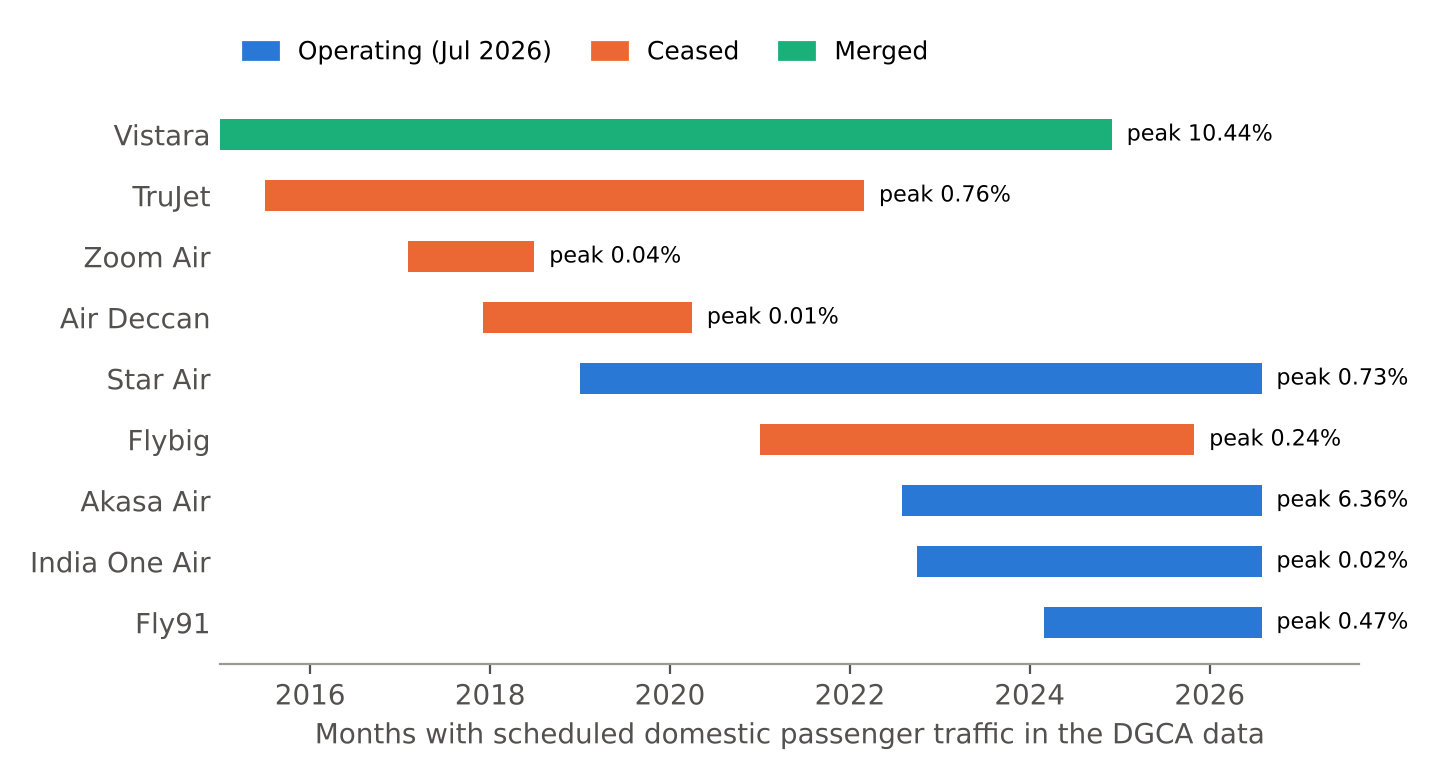
\includegraphics[width=0.92\textwidth]{figures/fig_o3_lifespans.png}
\captionof{figure}{O3: Operating span and peak passenger share of the nine entrants, January 2015--July 2026; colour shows the outcome at July 2026. Source: DGCA via Kubicek (2026); authors' calculations.}
\label{fig:o3-life}
\end{minipage}
\end{mergedcontribution}
\clearpage
\subsection{Route samples and concentration over time}
\label{app:eda-route-support}
The route evidence uses recovered DGCA schedules, pooling both directions of each airport pair. The entrant analysis retains airline brands and uses full-season departure totals alongside separate monthly records. The concentration analysis combines brands by ownership and follows a fixed top-20 sample. Table~\ref{tab:review-route-samples} distinguishes these samples rather than adding their counts together.

\begin{resultstable}{Samples drawn from the DGCA schedule archive.}{tab:review-route-samples}
\color{black}
\begin{tabular}{|>{\raggedright\arraybackslash}p{\dimexpr0.28\linewidth-2\tabcolsep-1.3333333333333333\arrayrulewidth\relax}|>{\raggedright\arraybackslash}p{\dimexpr0.38\linewidth-2\tabcolsep-1.3333333333333333\arrayrulewidth\relax}|>{\raggedright\arraybackslash}p{\dimexpr0.34\linewidth-2\tabcolsep-1.3333333333333333\arrayrulewidth\relax}|}
\hline
\textbf{Sample} & \textbf{Coverage} & \textbf{Observation} \\
\hline
Entrant full-season comparison & Nine entrants, 229 airline--airport-pair--season observations & All scheduled departures over the selected season \\
\hline
Entrant major-route series & 20 airport pairs, April 2019--July 2026 & Airline and airport pair in one month \\
\hline
TruJet regional extension & 30 airport pairs across 14 observed months in 2019--2022 & Airline and airport pair in one month \\
\hline
Ownership-group concentration panel & 20 fixed airport pairs, 1,150 retained observations across 66 available months, April 2019--September 2026 & Airport pair in one month \\
\hline
\end{tabular}
\par\vspace{5pt}{\footnotesize\setstretch{1.05}\raggedright \textbf{Note:} Each entrant uses its latest usable season before closure or merger, or its latest available season. Services are counted using their operating days and start and end dates. The top-20 sample is selected using 2025 passenger totals, with a top-ten subset. The samples overlap and have different units.\par\textbf{Source:} Sweta\textquotesingle s and Goutham\textquotesingle s DGCA schedule preparation and source descriptions.\par}
\end{resultstable}\begin{mergedcontribution}{authorGoutham}
Figure~\ref{fig:o4-route-heatmap} shows how HHI varies across individual airport pairs over time. Each row represents one airport pair and each column one calendar month. Colours use a common 0--10,000 HHI scale. Grey cells indicate unavailable data, and gaps are not interpolated.

\begin{figure}[H]
\centering
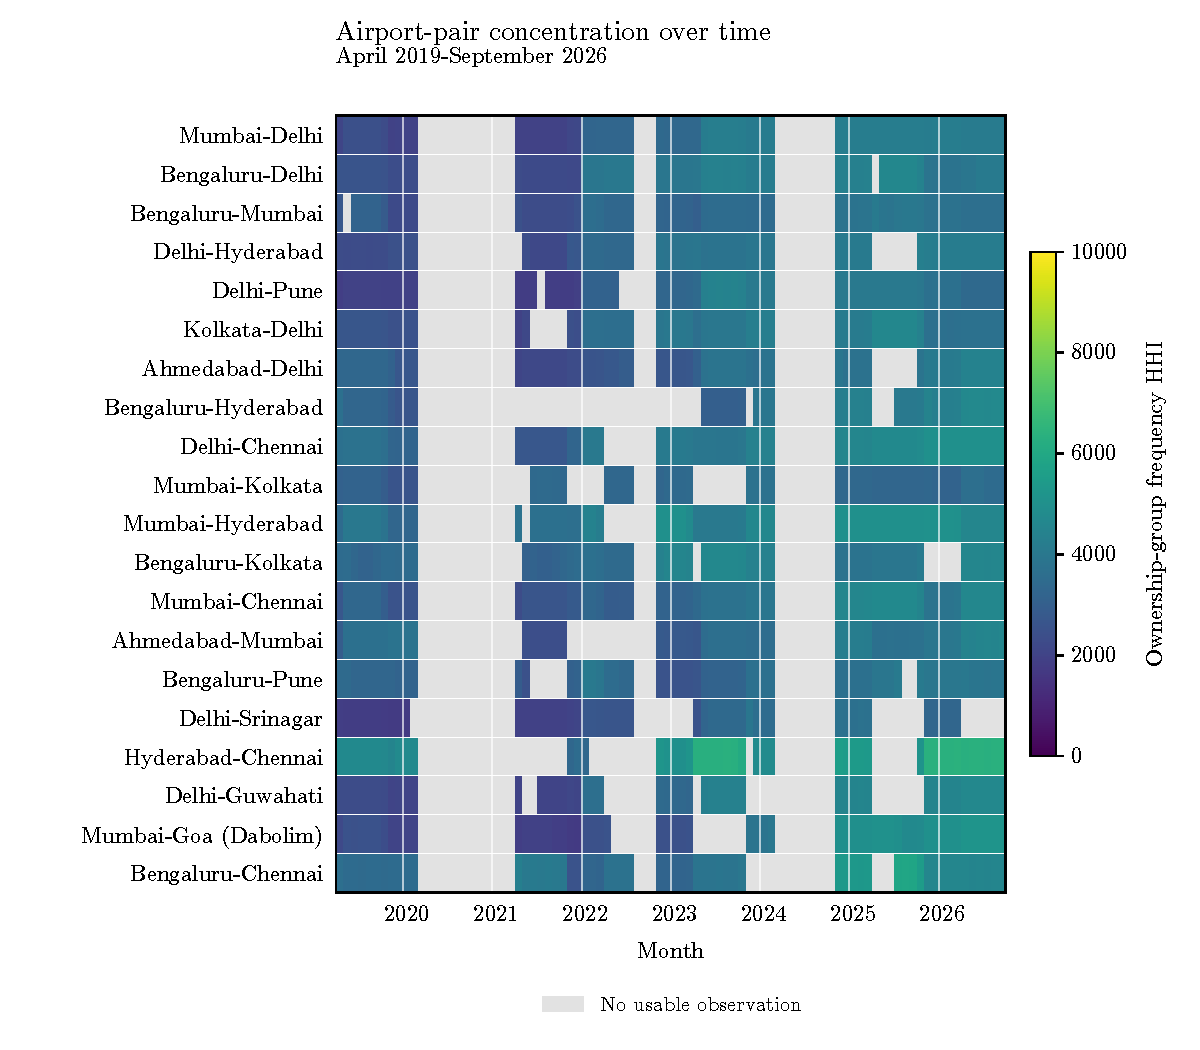
\includegraphics[width=\linewidth]{figures/o4_route_hhi_heatmap.pdf}
\caption{Ownership-group frequency HHI by airport pair and month.}
\label{fig:o4-route-heatmap}
\vspace{2pt}
\begin{minipage}{\linewidth}
\footnotesize\setstretch{1.1}
\textit{Source:} DGCA approved domestic schedules; authors' calculations.
\end{minipage}
\end{figure}
\end{mergedcontribution}
\clearpage
\subsection{Financial record coverage}
\label{app:eda-financial-coverage}
\begin{mergedcontribution}{authorSweta}
The financial evidence comes from company and rating reports, parliamentary replies and selected press reports. Coverage differs across airlines and years, and net results are kept separate from operating results. Table~\ref{tab:review-financial-coverage} describes the available inputs. Financial comparisons and calculated margins are in Section~\ref{sec:review-o3-results}.

\begin{resultstable}{Financial and funding records used in O3.}{tab:review-financial-coverage}
\color{authorSweta}
\begin{tabular}{|>{\raggedright\arraybackslash}p{\dimexpr0.27\linewidth-2\tabcolsep-1.3333333333333333\arrayrulewidth\relax}|>{\raggedright\arraybackslash}p{\dimexpr0.36\linewidth-2\tabcolsep-1.3333333333333333\arrayrulewidth\relax}|>{\raggedright\arraybackslash}p{\dimexpr0.37\linewidth-2\tabcolsep-1.3333333333333333\arrayrulewidth\relax}|}
\hline
\textbf{Source} & \textbf{Coverage} & \textbf{Available inputs} \\
\hline
ICRA rating reports & Vistara: FY2023--FY2024. Akasa Air: FY2025--FY2026. & Operating income, profit after tax and funding evidence \\
\hline
Lok Sabha reply, December 2025 & Available entrant records for FY2023--FY2025 & Reported profit or loss after tax, with provisional figures identified \\
\hline
DGCA operating results reported in Parliament & Available airline-year records for FY2017--FY2021 & Revenue and operating results, with revisions and provisional figures identified \\
\hline
Company releases and selected press reports & Airline-specific dates and financial years & Funding announcements, operating outcomes and additional revenue figures \\
\hline
\end{tabular}
\par\vspace{5pt}{\footnotesize\setstretch{1.05}\raggedright \textbf{Note:} These records do not form a balanced annual panel. Unavailable values are not zero, and different accounting bases are not pooled.\par\textbf{Source:} ICRA (2024, 2026), Ministry of Civil Aviation (2025), Rajya Sabha (2019, 2021), and the company/press records listed with the O3 references.\par}
\end{resultstable}
\end{mergedcontribution}
